\documentclass[a4paper,10pt]{article}
\usepackage[utf8]{inputenc}
\usepackage{amsmath}
\usepackage{amsfonts}
\usepackage{hyperref}
\usepackage{tikz}
\usetikzlibrary{decorations.pathreplacing}

\title{Interest Rate Modeling}
\author{Nathan NDJOLI - \href{mailto:nathan.ndjoli1@gmail.com}{nathan.ndjoli1@gmail.com}}
\date{July 2024}

\begin{document}

\maketitle

\section{Stochastic Processes}
\subsection{Markov Process}
\noindent A variable \( X(t) \) follows a Markov process if the values of \( X(t) \) for two time intervals \( \Delta t \) are independent. \\

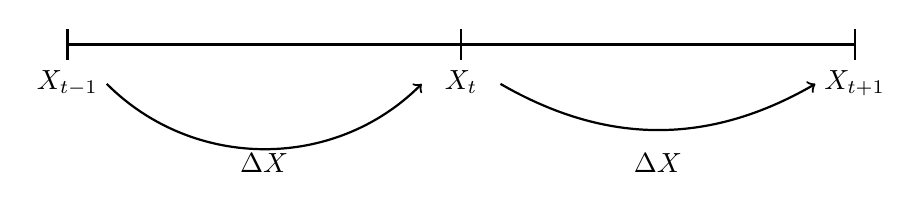
\begin{tikzpicture}
    % Draw the main line
    \draw[thick] (0,0) -- (10,0);

    % Draw the ticks and label them
    \draw[thick] (0,0.2) -- (0,-0.2) node[below] {\( X_{t-1} \)};
    \draw[thick] (5,0.2) -- (5,-0.2) node[below] {\( X_{t} \)};
    \draw[thick] (10,0.2) -- (10,-0.2) node[below] {\( X_{t+1} \)};

    % Draw the curved arrows
    \path[->,thick] (0.5, -0.5) edge[bend left=-45] (4.5, -0.5);
    \path[->,thick] (5.5, -0.5) edge[bend left=-30] (9.5, -0.5);
    
    % Labels for the curved arrows
    \node at (2.5, -1.5) {\(\Delta X\)};
    \node at (7.5, -1.5) {\(\Delta X\)};
    
\end{tikzpicture}\\

\noindent The intuition behind a Markov process is that it is a memoryless process. This means that the future state of the process depends only on the present state and not on past states. This characteristic is often associated with the notion of weak-form informational efficiency, where all available information is already incorporated into the current state. \\

\subsection{Brownian Motion}
\noindent A variable \( W(t) \) follows a standard Brownian motion if it meets the following two conditions: it follows a Markov process and the variation \( \Delta W(t) \) over a time interval \( \Delta t \) is given by \[ \Delta W(t) = \epsilon \sqrt{\Delta t}, \] where \( \epsilon \) follows a standard normal distribution \( N(0, 1) \). \\

\noindent The consequences of this definition are that the expected value of \( W(t) \) is zero, i.e., \[ E(\Delta W(t)) = E(\epsilon \sqrt{\Delta t}) = \sqrt{\Delta t} E(\epsilon) = 0, \] and that the variance of \( W(t) \) is proportional to time, i.e., \[ V(\Delta W(t)) = V(\epsilon \sqrt{\Delta t}) = \Delta t V(\epsilon) = \Delta t. \] Therefore, \( \Delta W(t) \) follows a normal distribution \( N(0, \sqrt{\Delta t}) \). \\

\noindent Consider an example where the initial value of a variable \( W(t) \) following a Brownian process is 12. We want to determine the distribution of \( W(t) \) after 4 years. We consider a relatively long period \( T \), with \( T = N \Delta t \). The variation of \( W(t) \) over this period is given by \[ W(T) - W(0). \] Thus, \[ W(T) - W(0) = \sum_{i=1}^{N} \Delta W(t) = \sum_{i=1}^{N} \epsilon \sqrt{\Delta t}. \] Consequently, \[ E(W(T) - W(0)) = \sum_{i=1}^{N} E(\epsilon \sqrt{\Delta t}) = 0, \] hence \[ E(W(T)) = W(0). \] Similarly, \[ V(W(T) - W(0)) = \sum_{i=1}^{N} V(\epsilon \sqrt{\Delta t}) = N \Delta t = T. \] Therefore, \( W(T) \) follows a normal distribution \( N(W(0), \sqrt{T}) \), which in this case implies: \( W(4) \) follows a normal distribution \( N(12, 2) \). \\

\subsection{Generalized Wiener Process}
\noindent A variable \( Y(t) \) follows a generalized Wiener process if it can be written as \[ \Delta Y(t) = a \Delta t + b \Delta W(t), \] where \( a \) and \( b \) are constants with \( b > 0 \). \\

\noindent The parameter \( a \), called the drift, measures the expected value of \( \Delta Y(t) \) per unit of time. In other words, \[ E(\Delta Y(t)) = a \Delta t + b E(\Delta W(t)) = a \Delta t. \] Thus, \[ a = \frac{E(\Delta Y(t))}{\Delta t}. \] \\

\noindent The parameter \( b^2 \), called the variance parameter, measures the variance of \( \Delta Y(t) \) per unit of time. Hence, \[ V(\Delta Y(t)) = V(a \Delta t) + V(b \Delta W(t)) = b^2 V(\Delta W(t)) = b^2 \Delta t. \] Therefore, \[ b^2 = \frac{V(\Delta Y(t))}{\Delta t}. \] \\

\noindent Consequently, \( \Delta Y(t) \) follows a normal distribution \( N(a \Delta t, b \sqrt{\Delta t}) \). \\

\noindent Consider the example where the variable \( Y(t) \) follows a Wiener process with a drift of 15 and a variance parameter of 100. The initial value of this variable is 20. We seek to determine the distribution of \( Y(t) \) after 9 years. The variation \( Y(T) - Y(0) \) can be expressed as the sum of the infinitesimal variations \( \Delta Y(t) \) over the considered time interval. Thus, \[ Y(T) - Y(0) = \sum_{i=1}^{N} \Delta Y(t). \] Consequently, \[ E(Y(T) - Y(0)) = \sum_{i=1}^{N} E(\Delta Y(t)) = N a \Delta t = a T, \] hence \[ E(Y(T)) = a T + Y(0). \] Similarly, \[ V(Y(T) - Y(0)) = \sum_{i=1}^{N} V(\Delta Y(t)) = N b^2 \Delta t = b^2 T. \] Therefore, \( Y(T) \) follows a normal distribution \( N(a T + Y(0), \sqrt{b^2 T}) \), which in this case implies: \( Y(9) \) follows a normal distribution \( N((9 \cdot 15) + 20, 30) \), i.e., \( N(155, 30) \). \\


\section{The Vasicek Model}

\noindent The Vasicek model is used for the modeling of interest rates. In this model, the instantaneous spot interest rate at date \( t \), denoted as \( r(t) \), follows an Ornstein-Uhlenbeck process. The differential equation describing this process is:
\[dr(t) = a(k - r(t))dt + \epsilon dW(t)\]
\noindent In this equation, \( \epsilon dW(t) \) represents a random shock, while \( a(k - r(t))dt \) acts as a mean-reverting force. This mean-reverting term ensures that if the interest rate \( r(t) \) is below the long-term mean \( k \), the force is positive, causing \( r(t) \) to increase towards \( k \). Conversely, if \( r(t) \) is above \( k \), the force is negative, pulling \( r(t) \) back down towards \( k \). \\

\subsection{Solving the differential equation}

\noindent To solve this differential equation for a future date \( u > t \), we obtain the following solution:
\[r(u) = r(t)e^{-a(u-t)} + k(1 - e^{-a(u-t)}) + \epsilon e^{-au} \int_{t}^{u} e^{az} dW(z)\]

\noindent This solution demonstrates that the interest rate \( r(u) \) at a future time \( u \) is normally distributed. The expected value and variance of \( r(u) \) are given by: 
\[E(r(u)) = r(t)e^{-a(u-t)} + k(1 - e^{-a(u-t)})\]
\[V(r(u)) = \frac{\epsilon^2}{2a} (1 - e^{-2a(u-t)})\]

\subsection{Value of the zero-coupon (ZC) bond}

\noindent Now consider a zero-coupon bond (ZC bond), which is a debt security without counterparty risk, paying 1 euro at maturity \( T \). The value of this bond at time \( t \) is denoted as \( P(t, T) \). It can be expressed as:
\[P(t, T) = e^{-(T-t)R(t,T)}\]

\subsection{Value of the ZC rate R(t, T)}

\noindent Here, \( R(t, T) \) represents the zero-coupon rate at time \( t \) for a bond maturing at \( T \). The zero-coupon rate \( R(t, T) \) is the average of the instantaneous rates \( r(u) \) over the interval from \( t \) to \( T \):
\[R(t, T) = \frac{1}{T - t} \int_{t}^{T} r(u) du\]

\noindent Thus, the bond price can be rewritten using the expected value of this expression, considering the stochastic nature of \( r(u) \):
\[P(t, T) = E\left[ e^{-\int_{t}^{T} r(u) du} \right]\]

\noindent The value of the zero-coupon bond at time \( t \) is then given by: 
\[P(t, T) = A(t, T)e^{-B(t,T)r(t)}\]

\noindent Where:
\[A(t, T) = e^{\left(k - \frac{\epsilon^2}{2a^2}\right)\left(B(t,T) - (T-t)\right) - \frac{\epsilon^2}{4a} B(t,T)^2}\]
\noindent And:
\[B(t, T) = \frac{1 - e^{-a(T-t)}}{a}\]\\

\noindent It should be noted that the price \( P(t, T) \) of the zero-coupon bond follows a log-normal distribution. \\

\noindent The zero-coupon rate \( R(t, T) \) can be determined from the bond price \( P(t, T) \) by the relation: 
\[R(t, T) = -\frac{1}{T - t} \ln P(t, T)\]

\noindent This relationship can be further expanded using the expressions for \( A(t, T) \) and \( B(t, T) \): 

\[R(t, T) = \frac{1}{T - t} \left[B(t, T)r(t) - \ln A(t, T)\right]\]\\

\noindent As the maturity \( T \) approaches infinity, the zero-coupon rate converges to a long-term mean rate \( R_\infty \), given by: 
\[\lim_{T \to \infty} R(t, T) = R_\infty = k - \frac{\epsilon^2}{2a^2}\]

\noindent By substituting the expressions for \( A(t, T) \) and \( B(t, T) \) into the formula for \( R(t, T) \), we obtain: 

\[R(t, T) = R_\infty + (r(t) - R_\infty) \frac{1 - e^{-a(T-t)}}{a(T - t)} + \frac{\epsilon^2}{4a^3(T - t)} \left[1 - e^{-a(T-t)}\right]^2\]

\subsection{Scope of the Vasicek model}

\noindent The Vasicek model has several important implications for the behavior of interest rates. One significant implication is that the short-term interest rate, or short rate, may not always be positive. This characteristic arises due to the mean-reverting nature of the Ornstein-Uhlenbeck process and the random shocks represented by \( \epsilon dW(t) \). When the mean-reverting force is weak or the volatility is high, there is a non-negligible probability that the short rate could become negative. While this feature captures the realistic possibility of very low or even negative interest rates observed in some economic conditions, it also introduces certain limitations in the model's practical application. For instance, the possibility of negative rates can complicate the pricing of interest rate derivatives and the valuation of fixed-income securities. Moreover, some financial instruments and contracts assume a non-negative interest rate, which may necessitate adjustments or alternative modeling approaches when using the Vasicek model in such contexts. \\

\subsection{Application to the Valuation of Bond Options}

\noindent In the context of options on bonds, we consider a specific type of option known as an option on a zero-coupon bond. This option has a strike price \( K \) and matures at time \( T \). The underlying asset is a zero-coupon bond with a nominal value of 1 euro, maturing at time \( T + D \). Zero-coupon bonds, unlike regular bonds, do not make periodic interest payments. Instead, they are sold at a discount to their face value and pay the full face value at maturity. The price of a zero-coupon bond is log-normally distributed, which is consistent with the Vasicek model's assumptions.\\

\noindent For a call option, the value \( C(t) \) at time \( t \) is given by: 
\[C(t) = P(t, T + D)N(d1) - KP(t, T)N(d2)\]\\
\noindent For a put option, the value \( P(t) \) at time \( t \) is given by:
\[P(t) = -P(t, T + D)N(-d1) + KP(t, T)N(-d2)\]
 \noindent With:\\\\
\noindent \( P(t, T + D) \): price at time \( t \) of the zero-coupon bond maturing at \( T + D \)\\
\newline \noindent \( P(t, T) \): price at time \( t \) of the zero-coupon bond maturing at \( T \). 

\noindent And:\\
\[d1 = \frac{\ln \frac{P(t, T + D)}{P(t, T)K} + \frac{\epsilon^2}{2} \ln P(T, T + D)}{\epsilon \ln P(T, T + D)}\]

\[d2 = d1 - \epsilon \ln P(T, T + D)\]\\

\noindent In these equations, \( \epsilon \ln P(T, T + D) \) is the volatility term and is calculated by:

\[\epsilon \ln P(T, T + D) = \epsilon \frac{1 - e^{-aD}}{a} \sqrt{\frac{1 - e^{-2a(T-t)}}{2a}}\]

\noindent These equations provide the necessary framework for evaluating the price of options on zero-coupon bonds within the Vasicek model. By substituting the appropriate values into these formulas, one can determine the fair price of both call and put options on zero-coupon bonds, taking into account the dynamics of interest rates as modeled by the Vasicek process. \\

\section{The Cox-Ingersoll-Ross (CIR) Model}

\noindent The Cox, Ingersoll, and Ross (CIR) model is used for the modeling of interest rates, addressing the issue of the positivity of rates. This model was proposed by Cox, J., Ingersoll, J., and Ross, S. in 1985 in their paper "A theory of the term structure of interest rates," published in Econometrica, volume 53, pages 385-407. \\

\noindent In the CIR model, the instantaneous spot interest rate at date \( t \) follows the process:
\[dr(t) = a(k - r(t))dt + \epsilon \sqrt{r(t)} dW(t)\]

\noindent This process differs from the Gaussian framework used in other models, particularly by eliminating the possibility of negative interest rates. If the interest rate reaches zero, the term \( \epsilon \sqrt{r(t)} dW(t) \) becomes zero, and only the term \( a(k - r(t))dt \) remains, ensuring that \( dr(t) = ak dt > 0 \). This means that the instantaneous interest rate cannot fall below zero, as zero acts as a "reflective barrier." \\

\subsection{Value of the zero-coupon (ZC) bond P(t,T)}

\noindent To evaluate the value of a zero-coupon bond (ZC bond) in this model, the value at time \( t \) of a bond maturing at \( T \) is given by:
\[P(t, T) = A(t, T) e^{-B(t, T) r(t)}\]

\noindent The difference from the Vasicek model lies in the expressions for \( A(t, T) \) and \( B(t, T) \). In the CIR model, we have:
\[A(t, T) = \left[ \frac{2\gamma e^{(a+\gamma)(T-t)/2}}{(a+\gamma)(e^{\gamma (T-t)}-1) + 2\gamma} \right]^{2ak/\epsilon^2}\]

\[B(t, T) = \frac{2(e^{\gamma (T-t)} - 1)}{(a+\gamma)(e^{\gamma (T-t)} - 1) + 2\gamma}\]

\noindent with:
\[\gamma = \sqrt{a^2 + 2\epsilon^2}\]\\

\subsection{Value of the ZC rate R(t, T)}

\noindent The value of the zero-coupon rate \( R(t, T) \) can be determined from the price of the zero-coupon bond \( P(t, T) \) by the relation:
\[R(t, T) = -\frac{1}{T - t} \ln P(t, T)\]

\noindent Thus,
\[R(t, T) = \frac{1}{T - t} \left[B(t, T) r(t) - \ln A(t, T)\right]\]\\

\noindent In the context of options on bonds, we consider a specific type of option known as an option on a zero-coupon bond. This option has a strike price \( K \) and matures at time \( T \). The underlying asset is a zero-coupon bond with a nominal value of 1 euro, maturing at time \( T + D \). Zero-coupon bonds, unlike regular bonds, do not make periodic interest payments. Instead, they are sold at a discount to their face value and pay the full face value at maturity. The price of a zero-coupon bond is log-normally distributed, which is consistent with the CIR model's assumptions.\\

\noindent For a call option, the value \( C(t) \) at time \( t \) is given by:
\[C(t) = P(t, T + D)N(d1) - KP(t, T)N(d2)\]

\noindent For a put option, the value \( P(t) \) at time \( t \) is given by:
\[P(t) = -P(t, T + D)N(-d1) + KP(t, T)N(-d2)\]

\noindent Here,
\[d1 = \frac{\ln \frac{P(t, T + D)}{P(t, T)K} + \frac{\epsilon^2}{2} \ln P(T, T + D)}{\epsilon \ln P(T, T + D)}\]
\[d2 = d1 - \epsilon \ln P(T, T + D)\]\\

\noindent In these equations, \( \epsilon \ln P(T, T + D) \) is the volatility term and is calculated by:
\[\epsilon \ln P(T, T + D) = \epsilon \frac{1 - e^{-aD}}{a} \sqrt{\frac{1 - e^{-2a(T-t)}}{2a}}\]

\noindent These equations provide the necessary framework for evaluating the price of options on zero-coupon bonds within the CIR model. By substituting the appropriate values into these formulas, one can determine the fair price of both call and put options on zero-coupon bonds, taking into account the dynamics of interest rates as modeled by the CIR process. \\

\section{The Hull-White Model}

\noindent The Hull-White model is used for the modeling of interest rates and is specifically designed to be compatible with the initial yield curve.\\

\noindent In the Hull-White model, the instantaneous spot interest rate at date \( t \), denoted as \( r(t) \), follows the stochastic differential equation:
\[dr(t) = (k(t) - ar(t))dt + \epsilon dW(t)\]

\noindent Here, \( k(t) \) is a time-dependent function that adjusts to ensure the model is consistent with the initial term structure of interest rates. The term \( ar(t) \) represents the mean-reverting force that pulls the interest rate towards the mean level, while \( \epsilon dW(t) \) introduces a random shock following a Wiener process \( W(t) \). \\

\noindent In the special case where \( k(t) = ak \), the process simplifies to:
\[dr(t) = (ak - ar(t))dt + \epsilon dW(t) = a(k - r(t))dt + \epsilon dW(t)\]
\noindent This special case is often referred to as the "extended Vasicek model" due to its similarity to the Vasicek interest rate model. \\

\subsection{Compatibility with the initial yield curve}

\noindent To ensure compatibility with the initial yield curve, the Hull-White model defines \( k(t) \) in terms of the instantaneous forward rate \( f_0(t) \), which is derived from the observed yield curve at time 0. The instantaneous forward rate \( f_0(t) \) is the rate applicable to an infinitesimally small time period starting at \( t \). \\

\noindent The model fits the observed yield curve at time 0 if:
\[k(t) = af_0(t) + f'_0(t) + \frac{\epsilon^2}{2a}(1 - e^{-2at})\]

\noindent In this expression, \( f'_0(t) \) is the slope of the instantaneous forward rate curve. The last term, \(\frac{\epsilon^2}{2a}(1 - e^{-2at})\), accounts for the adjustment due to the stochastic nature of interest rates, but it is often negligible. Hence, we can approximate \( k(t) \) as:
\[k(t) \approx af_0(t) + f'_0(t)\]

\noindent Therefore, the differential equation for the interest rate can be written as:
\[dr(t) \approx [af_0(t) + f'_0(t) - ar(t)]dt + \epsilon dW(t)\]

\noindent This leads to:
\[dr(t) \approx [a(f_0(t) - r(t)) + f'_0(t)]dt + \epsilon dW(t)\]

\noindent Consequently:
\begin{enumerate}
    \item If \( r(t) = f_0(t) \), then \( dr(t) = f'_0(t)dt + \epsilon dW(t) \). This indicates that the trend of the instantaneous spot rate follows the slope of the forward rate curve, meaning it remains equal to the forward rate.
    \item If \( r(t) < f_0(t) \), the mean-reverting force will pull the rate back up towards \( f_0(t) \).
\end{enumerate}

\subsection{Value of the ZC bond P(t, T)}

\noindent The valuation of zero-coupon bonds (ZC bonds) within the Hull-White model can be determined similarly to other interest rate models. The value of a zero-coupon bond at time \( t \) maturing at time \( T \) is given by:
\[P(t, T) = A(t, T)e^{-B(t, T)r(t)}\]

\noindent The difference from the Vasicek model lies in the expressions for \( A(t, T) \) and \( B(t, T) \). In the Hull-White model, these are defined as:
\[A(t, T) = \frac{P(0, T)}{P(0, t)}e^{B(t, T)f_0(t) - \frac{\epsilon^2}{4a}(1 - e^{-2at})B(t, T)^2}\]

\[B(t, T) = \frac{1 - e^{-a(T-t)}}{a}\]

\subsection{Comments}

\noindent There are several important aspects of the Hull-White model that make it a significant tool in the modeling of interest rates.

\begin{enumerate}
    \item The Hull-White model allows for the possibility of negative interest rates. This is due to the fact that the changes in the interest rate are normally distributed, which means there is a non-zero probability that the rate could fall below zero. This feature is particularly relevant in modern financial markets where negative interest rates have become a reality in some economies.
    
    \item The model operates within a Gaussian framework. This characteristic makes the Hull-White model analytically tractable, allowing for closed-form solutions for bond prices and other interest rate derivatives. The simplicity of the Gaussian framework facilitates easier implementation and calibration to market data, which is essential for practical applications.
    
    \item The valuation of options on bonds within the Hull-White model remains unchanged compared to other interest rate models. This means that the same pricing formulas that apply to other models can be used within the Hull-White framework. As a result, the Hull-White model can be seamlessly integrated into existing financial models and systems without requiring significant modifications.
    
    \item An important extension of the Hull-White model is the Heath, Jarrow, and Morton (HJM) model introduced in 1992. The HJM model provides a more generalized framework for modeling the evolution of interest rates over time. It extends the capabilities of the Hull-White model by allowing for a broader range of interest rate dynamics and accommodating a wider variety of market conditions. This extension enhances the flexibility and applicability of the Hull-White model in more complex financial environments.
\end{enumerate}



\end{document}